%
% tikztemplate.tex
%
% (c) 2018 Prof Dr Andreas Müller, Hochschule Rapperswil
%
\documentclass[tikz]{standalone}
\usepackage{times}
\usepackage{amsmath}
\usepackage{txfonts}
\usepackage[utf8]{inputenc}
\usepackage{graphics}
\usepackage{color}
\usepackage{pifont}
\usetikzlibrary{arrows,intersections,math,calc}
\begin{document}

\def\punkt#1{
        \fill[color=white] #1 circle[radius=0.08];
        \draw #1 circle[radius=0.08];
}

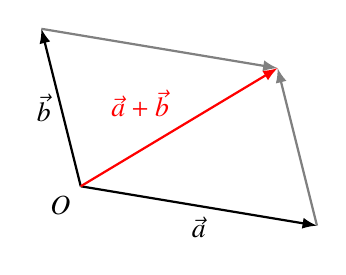
\begin{tikzpicture}[>=latex,thick]

\coordinate (O) at (0,0);
\coordinate (A) at (3,-0.5);
\coordinate (B) at (-0.5,2);
\coordinate (C) at ($(A)+(B)$);

\draw[->] (O)--(A);
\draw[->,color=gray] (A)--(C);
\draw[->] (O)--(B);
\draw[->,color=gray] (B)--(C);
\draw[->,color=red] (O)--(C);

%\node at (A) [below right] {$A$};
%\node at (B) [above left] {$B$};

\node at ($0.5*(A)$) [below] {$\vec{a}$};
\node at ($0.5*(B)$) [left] {$\vec{b}$};
\node[color=red] at ($0.5*(A)+0.5*(B)$) [above left] {$\vec{a}+\vec{b}$};

\punkt{(O)} \node at (O) [below left] {$O$};

\end{tikzpicture}

\end{document}

